\chapter{Motivação}

Vejamos algumas situações onde os objetos estudados nessa disciplina são usados.
\bigskip


\noindent\textbf{{\large Coordenadas Polares}}
	
\begin{itemize}
	\item \textbf{\color{blue}{Traçar curvas complexas}}
	\begin{figure}[h]
		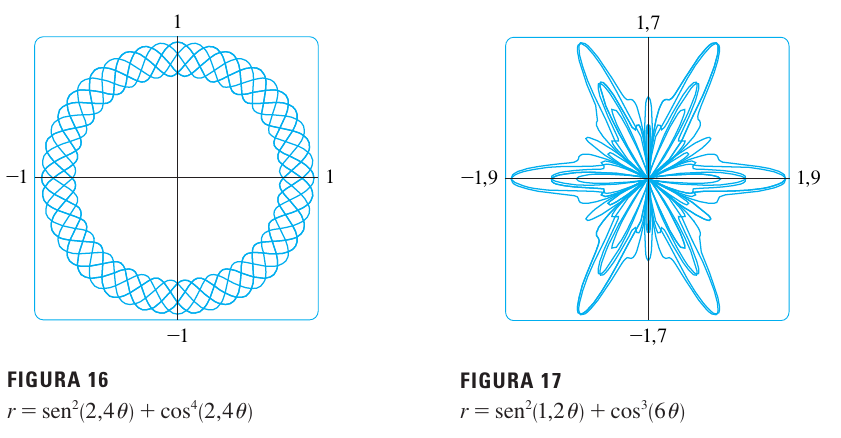
\includegraphics[scale=0.6]{figuras/introducao/curvas-polares1.png}
		\caption{}
	\end{figure}
	\item \textbf{{\color{blue}Aplicação na engenharia de som}}

Engenheiros de som usam coordenadas polares para descrever padrões de sons de microfones. Um padrão de captação em forma de {\color{blue}\textbf{cardioide}} captura principalmente a fonte sonora para a qual é apontado, como um cantor ou um instrumento, ao mesmo tempo que reduz a captação de ruído ambiente e sistemas de monitoramento de palco.

\begin{center}
	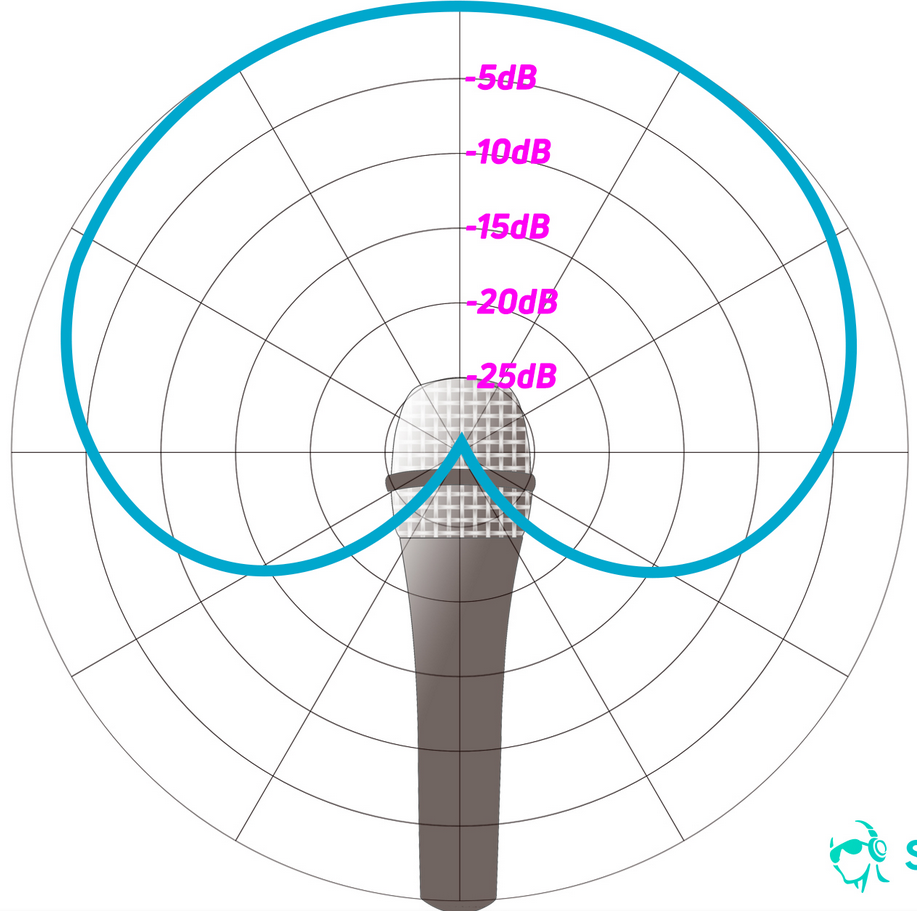
\includegraphics[scale=0.5]{figuras/introducao/cardioide-micro.png}
\end{center}
\end{itemize} 
	

\noindent\textbf{{\large Funções Vetoriais}}

\begin{itemize}
	\item \textbf{{\color{blue}Aplicação em Biologia}}
	
		Em 1953, James Watson e Francis Crick mostraram que a estrutura da molécula de
	{\color{blue}\textbf{DNA}} é de duas hélices circulares paralelas interligadas.

\begin{center}
	
\includegraphics[scale=0.7]{figuras/introducao/dna.png}
\end{center}



Sabendo-se o raio da hélice de DNA, o número de voltas e a altura de cada volta, usando o conceito de \dt{comprimento de curvas espaciais}, podemos calcular o comprimento da molécula de DNA.

\item \textbf{{\color{blue}Movimentos sobre curvas}}
	
No ensino médio, aprendemos que uma partícula em um  \dt{Movimento Circular Uniforme} tem velocidade constante {\color{teal} \(v\)}, mas para manter sua trajetória em um círculo de raio {\color{teal}\(R\)}, precisa de uma \dt{força centrípeta}, que gera a chamada \dt{aceleração centrípeta}, cuja fórmula é:
	\[
	{\color{teal} a_c=\frac{v^2}{R}}
	\]
	
	Contudo, para movimentos em um curva qualquer, essa aceleração tem uma \dt{forma vetorial}

	\[
	{\color{Goldenrod}\vec{a}}=v'\vec{T}+{\color{teal}\kappa v^2}\vec{N}
	\]

\begin{center}
	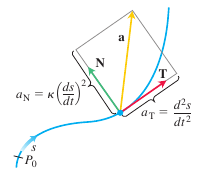
\includegraphics[scale=1.5]{figuras/introducao/curvatura.png}
\end{center}
\end{itemize}
\newpage

\noindent\textbf{{\large Funções de Várias Variáveis}}

\begin{itemize}
	\item \textbf{{\color{blue}Topografia}}
	
	As {\color{blue}curvas de nível} de funções de várias variáveis tem como exemplos de aplicações o estudo topográfico ou  das isotermas de regiões.
\begin{center}
	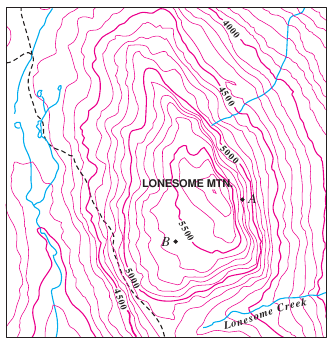
\includegraphics[scale=1]{figuras/nivel2.png}
\end{center}


\begin{center}
	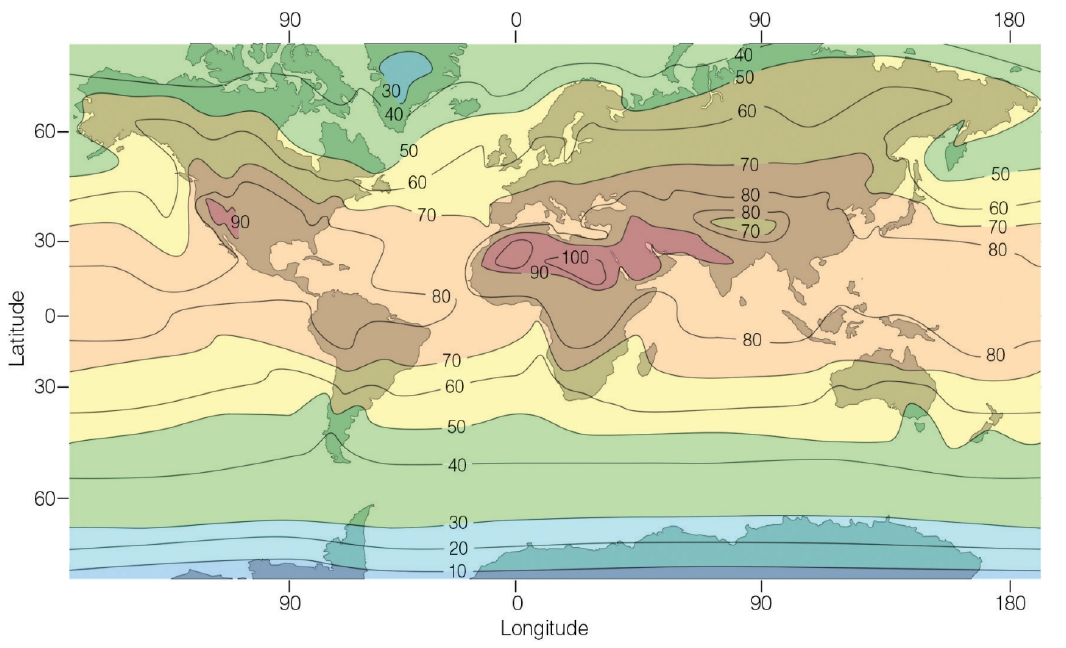
\includegraphics[scale=0.6]{figuras/nivel3.png}
\end{center}

\item \textbf{{\color{blue}Problema de Otimização: Produção restrita a um orçamento}}


A produção total \(P\) de certo produto depende do {\color{blue}custo \(x\) de trabalho empregado}  e da {\color{red}quantidade \(y\) de capital investido}. Na década de 1920 Charles
Cobb e Paul Douglas obtiveram o seguinte modelo
\[
P=b{\color{blue}x}^\alpha {\color{red}y}^{1-\alpha},
\]
onde \(b\) e \(\alpha\) são constantes positivas e \(\alpha<1\).

Para uma firma com função de produção e restrição orçamentária dadas por
\[
\begin{cases}
	P={\color{blue}x}^{2/3} {\color{red}y}^{1/3}\\
	{\color{blue}x}+ {\color{red}y}=3.78.
\end{cases}
\]
Teremos produção máxima \(P=2\) quando \({\color{blue}x=2.52}\) e \( {\color{red}y=1.26}\)
\begin{center}
	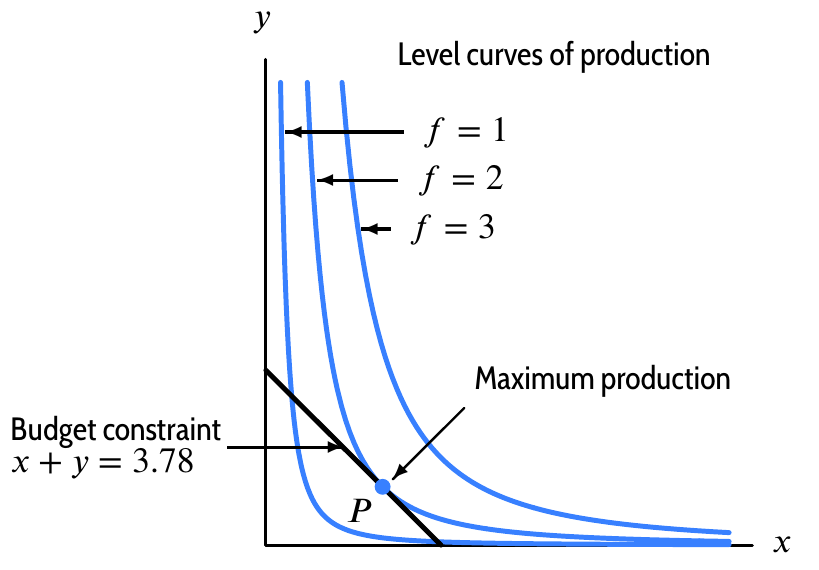
\includegraphics[scale=.7]{figuras/introducao/cobb-res.png}
\end{center}

\end{itemize}



